\subsection{\rich Mirror Alignment}
\textcolor{red}{This should include, description of the method (detector description
should be included in previous section), data selected, time required 
for this task, performance (before/after alignment) and stability of the constants. 
The overall performance, maybe also stability of the overall performance (PID 
or/and cherenkov angle resolution) could be together for calibration and alignment.}



Both \rich detectors have two sets of mirrors: photons are reflected off a
primary mirror onto a secondary mirror, from where they are deflected out of the
LHCb acceptance onto the photodetector plane.
\begin{figure}[h]
\begin{center}
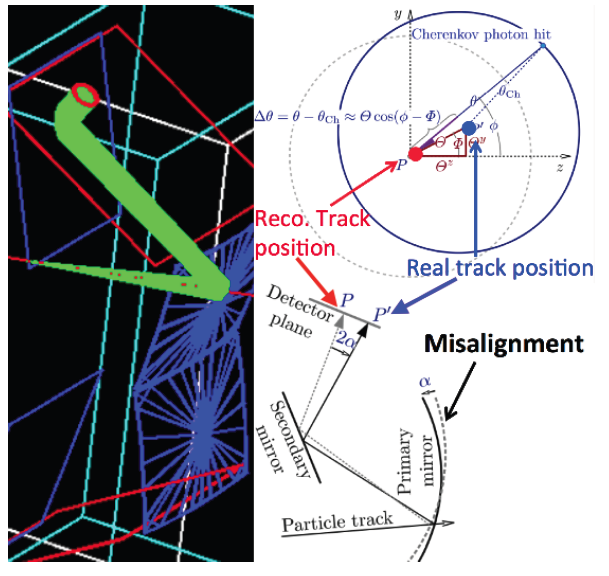
\includegraphics[width=0.7\textwidth]{../figures/RichMissAlign.png}
\caption{\label{fig:RichMissAlign} Left: 3D representation of a track (red line) going through a radiator and emitting Cherenkov photons (green cone). The photons are reflected by a spherical primary mirror (blue rectangle with star-shaped pattern) onto a flat secondary mirror (blue rectangle) and from there onto the photodetector plane (red rectangle). The observable Cherenkov ring is shown as a red circle on the photodetector plane. Right: Schematic illustration of the effects of a misalignment in the \rich mirror system. The projected track position on the photodetector plane $P$ is displaced by $\varTheta^z$ and $\varTheta^y$ with respect to the the actual center of the Cherenkov ring on the photodetector plane $P'$. The Cherenkov angle $\theta$ is evaluated relative to $P$ and varies with the azimuthal angle $\phi$.}
\end{center}
\end{figure}

Any misalignment of the \rich detectors with respect to the tracking system is observed as a shift of the track projection point on the photodetector plane from the center of its corresponding Cherenkov ring as is illustrated in Figure \ref{fig:RichMissAlign}. This shift is observed by analysing the Cherenkov angle, $\theta$, as a function of the azimuthal Cherenkov angle $\phi$, defined as the angle of the pixel hit in the coordinate system of the photodetector plane, with the projected track coordinate at the origin. For a well aligned detector the angle $\theta$ is independent of the angle $\phi$, whilst a misaligned system results in a sinusoidal distribution as shown in Figure \ref{fig:RichMirror}.\\
In practice, distributions of $\Delta \theta$ against $\phi$ are plotted for each possible combination of primary and secondary mirror, where $\Delta \theta (\phi) = \theta(\phi) - \theta_{\mathrm{Ch}}$ and $\theta_{\mathrm{Ch}}$ is the Cherenkov angle calculated from the momentum of the track and the refractive index of the radiator \cite{LHCb-DP-2012-003}. Any systematic shift away from the value $\theta_{\mathrm{Ch}}$ is observable as a shift in $\Delta \theta$. \\
The $\Delta \theta$ distribution is then divided into slices in $\phi$. For each slice, a one dimensional histogram of $\Delta \theta$ is fitted with a Gaussian plus a second order polynomial background, where the means of the Gaussians of the different slices are connected in the fit by a sinusoidal distribution given by 
\begin{equation}
\begin{aligned}
 \Delta \theta_{p,s} (\phi) & \equiv   [\theta(\phi)-\theta_{\mathrm{Ch}} ]_{p,s} \\
                            &    =         \varTheta^z_{p,s}\cos\phi
                                 +         \varTheta^y_{p,s}\sin\phi                 \\
\end{aligned}
\end{equation}
The final fit is shown in Figure \ref{fig:RichMirror}; the extracted values of $\varTheta^y_{p,s}$ and $\varTheta^z_{p,s}$ correspond to the misalignment on the  photodetector plane for a mirror combination of primary mirror $p$ and secondary mirror $s$ in the $y$ and $z$ direction respectively.\\
The alignment of the mirror segments has the extra complication that every photon is reflected twice, and thus the data must be separated into samples which have unique primary and secondary mirror combinations. For this procedure, only photons that can be uniquely associated to a given mirror combination are used. \\
%Mirror segments are identified by considering photons to have been emitted at both the start and end of the gas radiators. If the mirror segments reflecting the photons are the same in both cases, the photon trajectory is considered \textit{unambiguous} and is used for the alignment of mirror segments.\\
The mirror arrangement in \richone allows for alignment using a sequential approach, where the primary mirrors are aligned first, followed by the secondary mirrors. This is possible because photons reaching a particular secondary mirror can only be reflected from a single primary mirror. In \richtwo the larger number of primary/secondary mirror combinations makes the use of a sequential method impossible. The alignment of the \richtwo mirror segments is performed by solving a set of simultaneous equations to extract all the alignment parameters of all the mirrors. In general two iterations of this method are required to obtain the final mirror alignment.\\
\\
\begin{figure}[h]
\begin{minipage}{0.5\columnwidth}
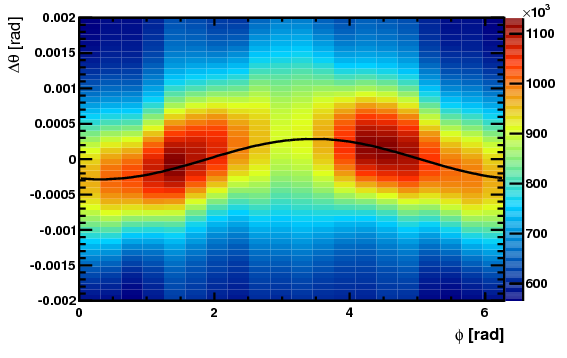
\includegraphics[width=\columnwidth]{../figures/RichMirror1.png}
\end{minipage}\hspace{2pc}%
\begin{minipage}{0.5\columnwidth}
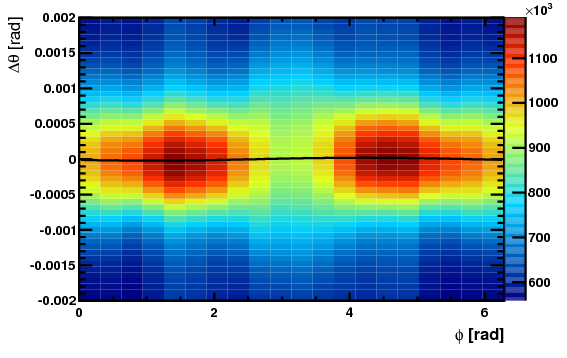
\includegraphics[width=\columnwidth]{../figures/RichMirror2.png}
\end{minipage} 
\caption{\label{fig:RichMirror} Difference between the measured and
  expected Cherenkov angle $\Delta\Theta$ as a function of the azimuthal angle $\phi$ before
  (left) and after (right) the mirror alignment for one mirror \cite{LHCb-DP-2012-003}.}
\end{figure}
As for the tracker alignment, the \richone and \richtwo alignments are performed on events collected by their respective \hltone lines. The \hltone lines for the \rich alignments trigger on high energy tracks whose Cherenkov photons would populate the outermost mirror combinations. The other mirror combinations are populated by the other tracks in the events. All tracks entering the alignment procedure have to have a momentum $p$ greater than 20(40)\gev for \richone (\richtwo) in order for the Cherenkov angle to be saturated and therefore $\theta_{\mathrm{Ch}}$ be predictable from the track momentum and the refractive index of the radiator.\\
The event reconstruction and filling of the $\Delta \theta$ vs. $\phi$ histograms is done by the analysers in parallel. The individual histograms are collected and merged and then fitted by the iterator. The iterator also determines the individual mirror misalignments and creates a new database slice with the mirror orientations and decided weather the alignment procedure has converged or if another iteration needs to be started. The alignment procedure takes about XXX for \richone and XXX for \richtwo.\\
MORE ON STABILITY AND PERFORMANCE TO COME SOON.\\